\section{Introduction}
\label{sec:intro}

\subsection{Standard model of particle physics}
\onehalfspacing The standard model (SM) of particle physics is so far the best theoretical model to describe the interaction of elementary 
particles using three of the four fundamental forces of nature which are electromagnetic force, strong nuclear force and the weak nuclear force. Gravitational force is neglected as the strength of this force is very weak at the scales over which elementary particle interact with each other. The standard model (SM) of particle physics is divided into two categories, bosonic sector and fermionic sector. Bosonic sector contain particles called bosons which mediate the fundamental forces of nature and the fermionic sector contain particles called fermions which make up all the matter in our universe. SM has three generations of matter (fermions) particles. The first generation of fermions consists of up (u) quark, down (d) quark, electron and electron neutrino, second generation consist of charm (c) quark, strange (s) quark, muon and muon neutrino and the third generation of matter particles has top (t) quark, bottom (b) quark, tau and tau neutrino. The bosonic sector consist of gauge bosons like gluon, photon, $W^{\pm}$, $Z^0$ which mediate strong nuclear force, electromagnetic force and weak nuclear force respectively. There is one more particle in the standard model called the Higgs Boson which gives mass to SM particles via electroweak symmetry breaking mechanism \cite{Chatrchyan:2012xdj}. All the standard model particles are shown in Figure 1. Higgs boson can be produced at the particle colliders like the Large Hadron Collider (LHC) in Geneva, Switzerland. \\

\begin{figure}[H]
  \centering
  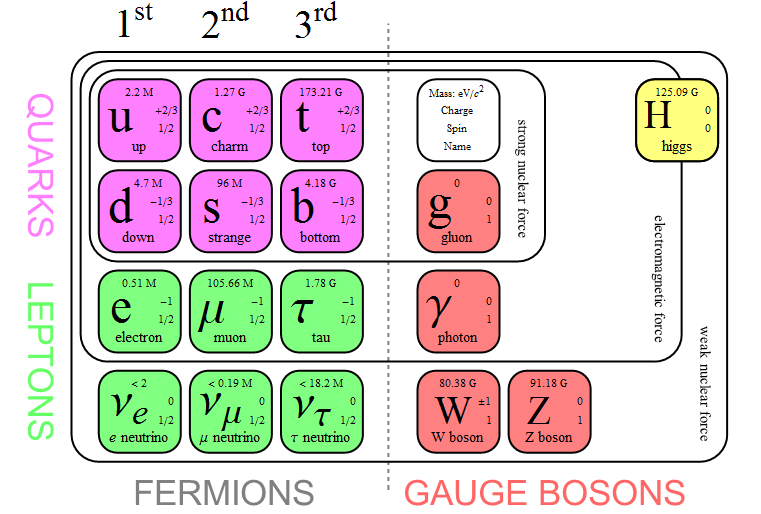
\includegraphics[width=0.7\columnwidth]{./SM.png}
  \caption{\onehalfspacing Standard model of particle physics showing matter and force carrier particles \cite{smpp}.}
  \label{fig:LHC}
\end{figure}


\subsection{Projections for Phase II High Luminosity (HL)-LHC}
LHC during the first run in 2011 and 2012 reached a peak instantaneous luminosity of 0.77 $\times$ $10^{34}$ $cm^{-2}s^{-1}$ which was more than 75$\%$ of its design luminosity and delivered an integrated luminosity of about 30 $fb^{-1}$ to each ATLAS and CMS. The LHC will deliver about 300 $fb^{-1}$ by 2024 \cite{collaborations2019report}. The goal of subsequently run of LHC has been to obtain datasets at higher values of luminosities for precision measurements of the properties of Higgs boson, in order to test the Standard Model pattern of couplings to elementary particles. In order to minimize the machine downtimes and maximize the productive use of the LHC for physics, the replacement of the inner triplet magnets (the one responsible to squeeze the beam at collision) and  of  all  hardware  changes  needed  to  enable  an  ambitious  luminosity  upgrade  will  take  place in parallel during one shutdown, at around 2023-25 (LS3), with some of the modification anticipated in 2019-2020 (LS2). This new phase of the LHC life has been named as High Luminosity LHC (HL-LHC) and has the scope of attaining the astonishing threshold of 3000 $fb^{-1}$ by the year 2036 as shown in Fig. 6. Figure 2 shows a summary of the projected uncertainties in the Higgs boson coupling parameters for Phase II HL-LHC using ggF, VBF, VH, and ${t\bar{t}H}$ production modes where luminosity is one of the dominant uncertainty in Higgs boson coupling measurement \cite{Tanabashi:2018oca}. \\





\begin{figure}[H]
  \centering
  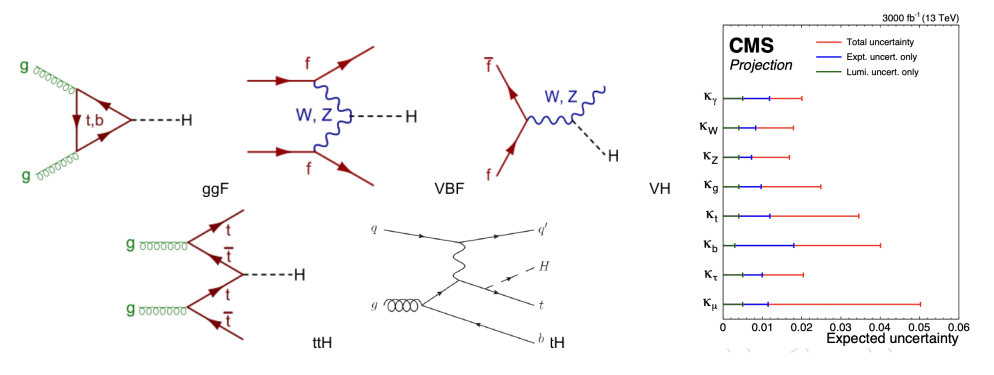
\includegraphics[width=1 \columnwidth]{./hig_pro.png}
  \caption{\onehalfspacing Left: Main production mechanisms for the Higgs boson at the LHC: gluon-gluon fusion (ggF), vector-boson fusion (VBF), associated vector boson (VH), associated top-quark pair (ttH), and associated single-top quark production (tH). Right: Expected uncertainties on the Higgs coupling parameters for 3000 $fb^{-1}$ of proton-proton collision data at 13 TeV center-of-mass energy \cite{Tanabashi:2018oca}.}
  \label{fig:LHC}
\end{figure}
